\documentclass[12pt,english,a4paper]{report}

\usepackage[utf8]{inputenc}          % Allows UTF-8 encoded characters in the .tex-file.
\usepackage{babel,csquotes,textcomp,duomasterforside} % Set LaTeX to structure the content following international academic standards.

\usepackage[toc,page]{appendix}

\usepackage{hyperref}
\usepackage{graphicx}
\usepackage{pdfpages}
\usepackage{listings}
\usepackage{wrapfig}
\usepackage{color,colortbl}
\usepackage{lettrine}
\usepackage[font={small,it}]{caption}
\usepackage{multirow}
\usepackage{tabularx}
\usepackage{footnote}
\usepackage{subfiles}
\usepackage{minted}
\usepackage{fancyvrb}
\usemintedstyle{friendly}

\newmintedfile[pythoncode]{python}{
fontsize=\scriptsize,
fontfamily=tt,
linenos=true,
numberblanklines=true,
numbersep=12pt,
numbersep=5pt,
gobble=0,
frame=leftline,
framerule=0.4pt,
framesep=2mm,
funcnamehighlighting=true,
tabsize=4,
obeytabs=false,
mathescape=false
samepage=false, %with this setting you can force the list to appear on the same page
showspaces=false,
showtabs =false,
texcl=false,
%breaklines = true
}

\newmintedfile[ccode]{c}{
fontsize=\scriptsize,
fontfamily=tt,
linenos=true,
numberblanklines=true,
numbersep=12pt,
numbersep=5pt,
gobble=0,
frame=leftline,
framerule=0.4pt,
framesep=2mm,
funcnamehighlighting=true,
tabsize=4,
obeytabs=false,
mathescape=false
samepage=false, %with this setting you can force the list to appear on the same page
showspaces=false,
showtabs =false,
texcl=false,
%breaklines = true
}

\newmintedfile[makecode]{make}{
fontsize=\scriptsize,
fontfamily=tt,
linenos=true,
numberblanklines=true,
numbersep=12pt,
numbersep=5pt,
gobble=0,
frame=leftline,
framerule=0.4pt,
framesep=2mm,
funcnamehighlighting=true,
tabsize=4,
obeytabs=false,
mathescape=false
samepage=false, %with this setting you can force the list to appear on the same page
showspaces=false,
showtabs =false,
texcl=false,
%breaklines =true
}

% Making the whole paragraph biz possible
%\usepackage{titlesec}
%\setcounter{secnumdepth}{4}
%\titleformat{\paragraph}
%{\normalfont\normalsize\bfseries}{\theparagraph}{1em}{}
%\titlespacing*{\paragraph}
%{0pt}{3.25ex plus 1ex minus .2ex}{1.5ex plus .2ex}

% Adding the bib
\usepackage[
    backend=biber,
    style=numeric
]{biblatex}
\addbibresource{refs.bib}

\definecolor{mygreen}{rgb}{0,0.6,0}
\definecolor{mygray}{rgb}{0.5,0.5,0.5}
\definecolor{mymauve}{rgb}{0.58,0,0.82}
\definecolor{auxiliryc}{RGB}{70,240,161} %Green
\definecolor{ineffectivec}{RGB}{70,149,240} %purple
\definecolor{effectivec}{RGB}{115,70,240} % Blue

\graphicspath{{./graphics/}}

% Setting tty font?
%\lstset{ %
%  basicstyle=\ttfamily\small,     
%  backgroundcolor=\color{white},   % choose the background color
%  breaklines=true,                 % automatic line breaking only at whitespace
%  captionpos=b,                    % sets the caption-position to bottom
%  commentstyle=\color{mygreen},    % comment style
%  escapeinside={\%*}{*)},          % if you want to add LaTeX within your code
%  keywordstyle=\color{blue},       % keyword style
%  stringstyle=\color{mymauve},     % string literal style
%  showspaces=false,
%  showstringspaces=false,
%}

\lstset{language=C,
  basicstyle=\ttfamily\scriptsize,
  keywordstyle=\color{blue}\ttfamily,
  stringstyle=\color{red}\ttfamily,
  commentstyle=\color{green}\ttfamily,
  breaklines=true,
  showspaces=false,
  showstringspaces=false,
  numbers=left,                    % where to put the line-numbers; possible values are (none, left, right)
  numbersep=5pt,    
  frame=single,                 % how far the line-numbers are from the code
  numberstyle=\tiny\color{mygray}, % the style that is used for the line-numbers
  rulecolor=\color{black}         % if not set, the frame-color may be changed on line-breaks 
}

\newenvironment{code}{\captionsetup{type=listing}}{}

\title{GPS Time Spoofing}
\subtitle{A detection and mitigation system for GPS timing}
\author{Aril Schultzen}
\begin{document}
\duoforside[dept={Institutt for informatikk},
program={Informatikk: programmering og nettverk},
long]

\begin{abstract}
Abstract goes here.
\end{abstract}

\chapter*{Foreword}
Here goes foreword

% Hackish code to keep counters and white pages at bay
\thispagestyle{empty}
\setcounter{page}{0}
\tableofcontents
\thispagestyle{empty}
\setcounter{page}{0}
\thispagestyle{empty}
\setcounter{page}{0}
\clearpage
\setcounter{page}{1}

% Here goes all the chapters
% ==================================================

\subfile{intro}

% Chapter about the csac and it's connectivity?

\chapter{Hardware}

\section{Chip Scale Atomic Clock}
I propose to use the Symmetricom SA.45 as the CSAC. This is a CSAC measuring only 16cc with 1 pulse per second (PPS) output and 1 PPS input (for disciplining). The SA.45's strength is it's low power consumption (less than 120mW) and low price \cite{SADS}. The SA.45 also uses a built-in controller which can be communicated with over a RS-232 serial interface. The ability to communicate with the CSAC, issue commands and collect data, is paramount for the feasibility of our proposal. It's worth mentioning that any atomic clock such as Cesium standard or even a Rubidium standard could be used given that they have a means to communicate basic telemetry as used by the SMACC software.

\section{SMACC platform}
I propose to use the Raspberry Pi 3 Model B (RASPI3) in the role as the host running the SMACC software. The RASPI3 is an interesting piece of equipment with an impressive list of specifications. It is a single board computer with a 1.2GHz 64-bit quad-core ARMv8 CPU, 1 GB of RAM, built in 802.11n Wireless LAN and four USB ports (\cite{RASPI}) (just to mention some). As with the Symmetricom SA.45, the RASPI3 is very affordable and retailed at about 35 USD when this report was written. We also propose to use Raspbian (\cite{RASPBIAN}), a Debian derived flavor of Linux optimized for the Raspberry Pi as the operating system. 

\section{GNSS receiver}
I propose to use at least two GNSS receivers. Both of the receivers should simply collect data and feed it to the SMACC but one of the receivers should also double as a 1 PPS disciplining source for the CSAC. Considering that need for a stable 1 PPS source, I propose to use the u-blox NEO-M8T. This is a relativity affordable GNSS receiver with a temperature compensated crystal oscillator (TCXO), 3 concurrent GNSS reception and an external antenna (\cite{UBLOXM8T}). Currently, only strings of NMEA data is collected from the GNSS receiver. However in the future it might be beneficial to collect and process raw data from the receivers as well. Since most GNSS receivers today follow the NMEA standard (to some extent) and raw data currently isn't required, common and popular receivers like the u-blox NEO-NEO series should be more that sufficient to use in an implementation if this proposal.

\chapter{Software}
\section{The Sensor Server/Client model}
Numerous approaches where considered when planning the implementation of the SMACC software (See \ref{da} for alternate approaches). The approach that was chosen is a Client/Server model which I have named the "Sensor Server". The Sensor Server model is based on the idea that a GNSS receiver and a computer can be viewed abstractly as a single device, a Sensor. The Server and Sensor communicates over an IP network. The Sensor runs a trivial program that receives data from a GNSS receiver, formats the data correctly and sends the data to a Server (more about the client \ref{sensor_client}). The Server on the other hand, is responsible for the heavy lifting. The data gathered from the Sensors are applied to what we call \textit{filters}. The filters are just algorithms that are able to detect anomalies in the data, thus making it possible to react to a spoofing or jamming attempt. Server tasks include:
\begin{itemize}
  \item Handle connections to all Sensors.
  \item Update structures as Sensor status changes (Disconnects, kick request)
  \item Communication with the CSAC and CSAC model updating
  \item Sensor data analysis and filter updates
  \item Raising alarms based on filter status
\end{itemize}
By using already existing network infrastructure, it becomes a lot easier to distribute Sensors and cover more area. This makes spoofing attacks harder to implement and easier to detect(\ref{cspakp}).However, every router and switch between a Sensor and the Server imposes a delay on the stream of packets between the two, especially when compared with a directly cabled approach. This might make the Sensor Server approach less responsive. It is of our understanding that whatever increase in complexity the Client/Server introduces to our approach, the Sensor Server makes up for by eliminating the need for potential miles of signal cables and signal amplifiers. 

\begin{figure}\label{server_core}
\centering
  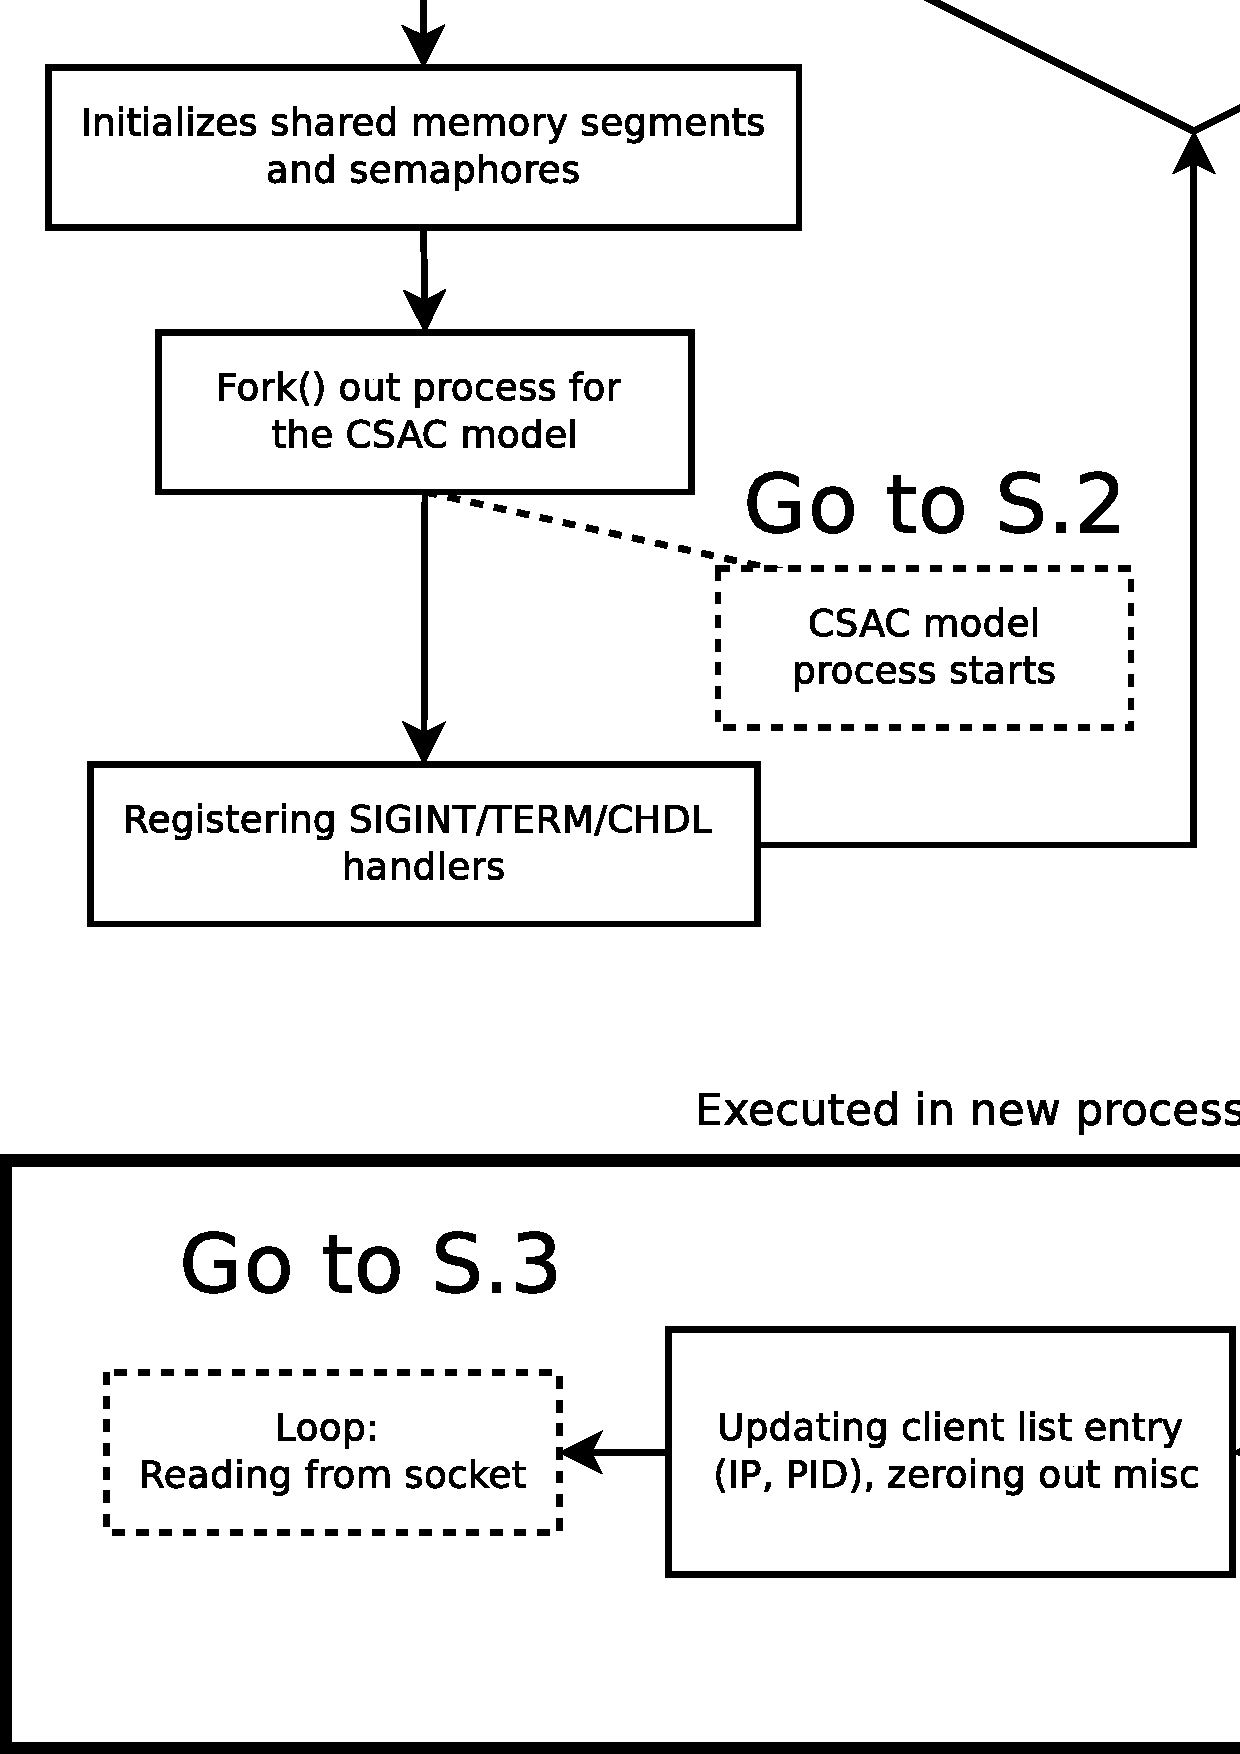
\includegraphics[scale=0.3]{server_core.pdf}
   \caption[Socket Server execution flow block diagram]{The block diagram shows an abstracted view of the Sensor Server.}
\end{figure}

\begin{figure}\label{server_flow}
\centering
  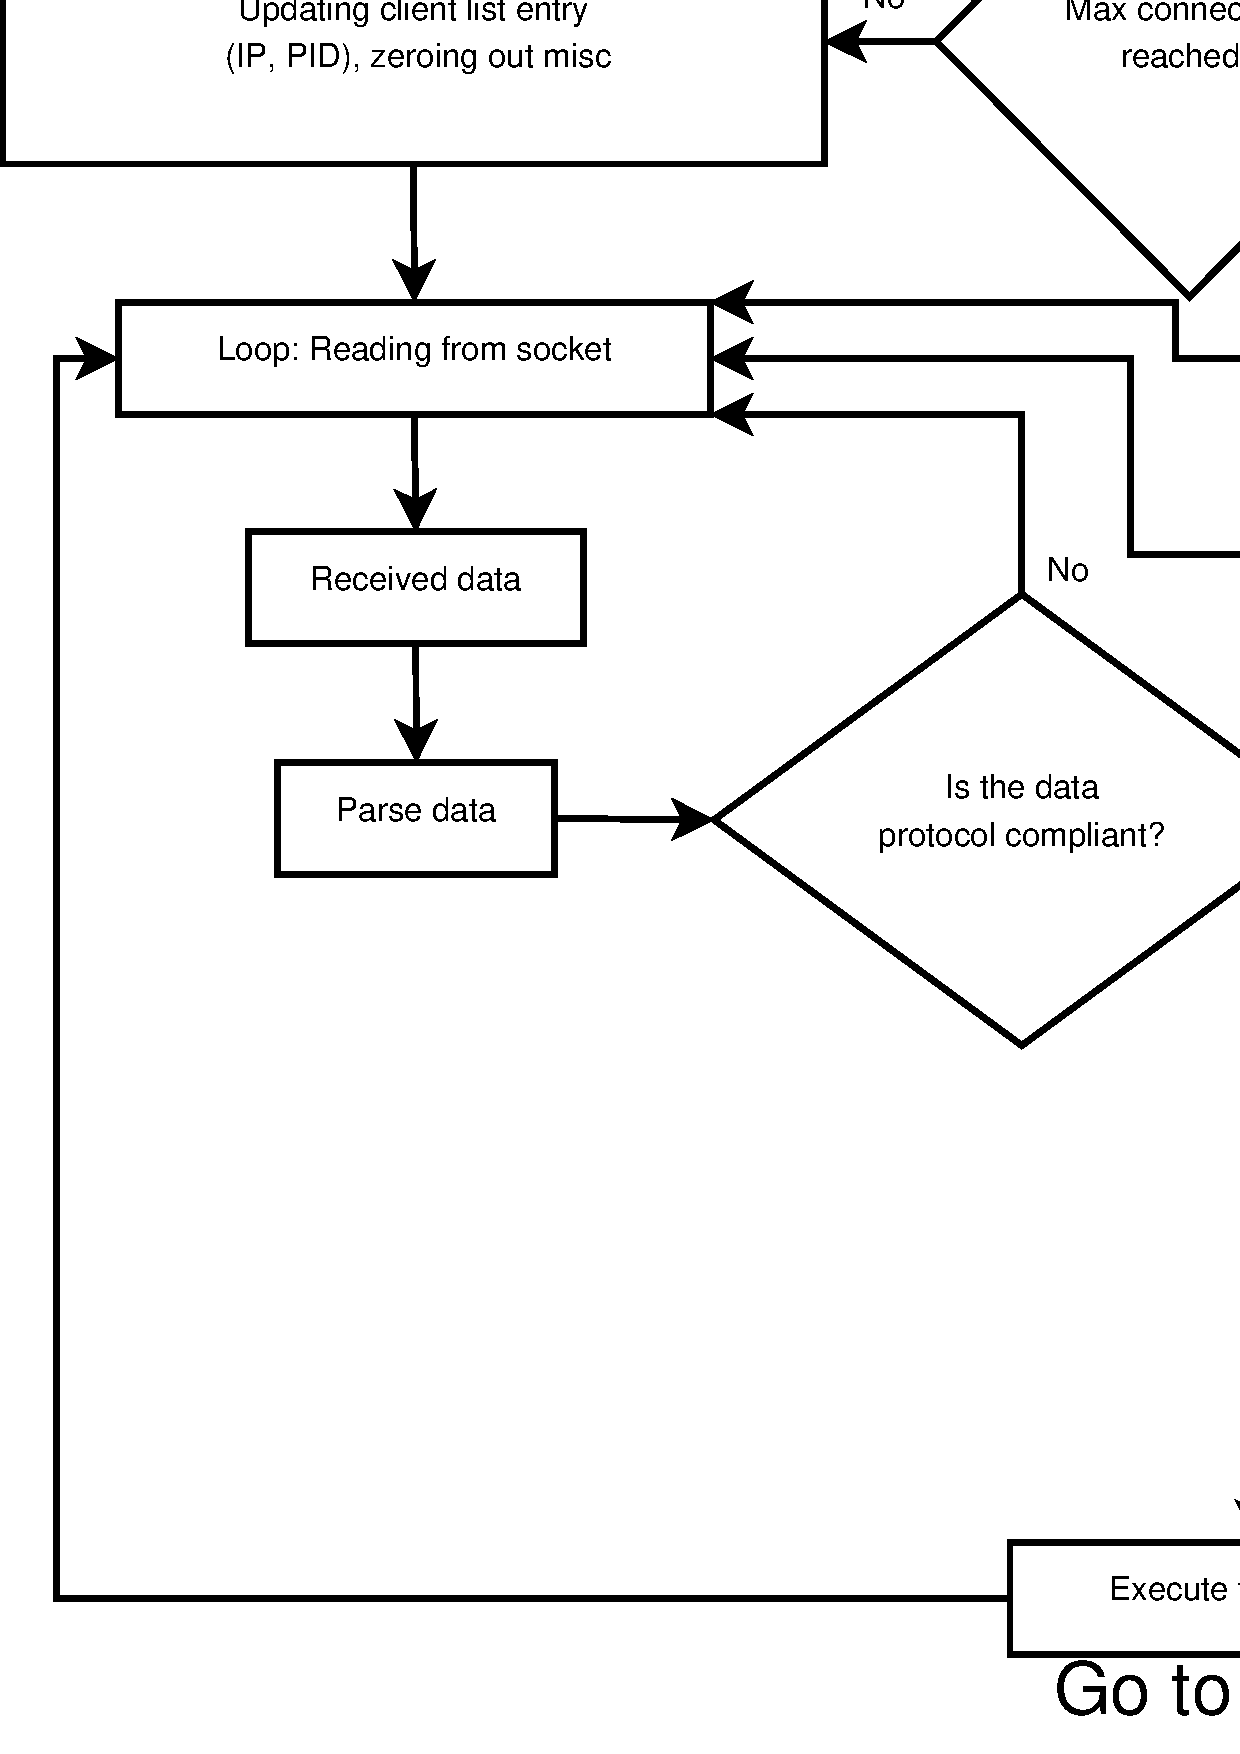
\includegraphics[angle=90, scale=0.3]{server_flow.pdf}
   \caption[Socket Server execution flow block diagram]{The block diagram shows an abstracted view of execution after a client has connected to the server and a \texttt{fork()} has been performed.}
\end{figure}

\begin{figure}\label{csac_filter}
\centering
  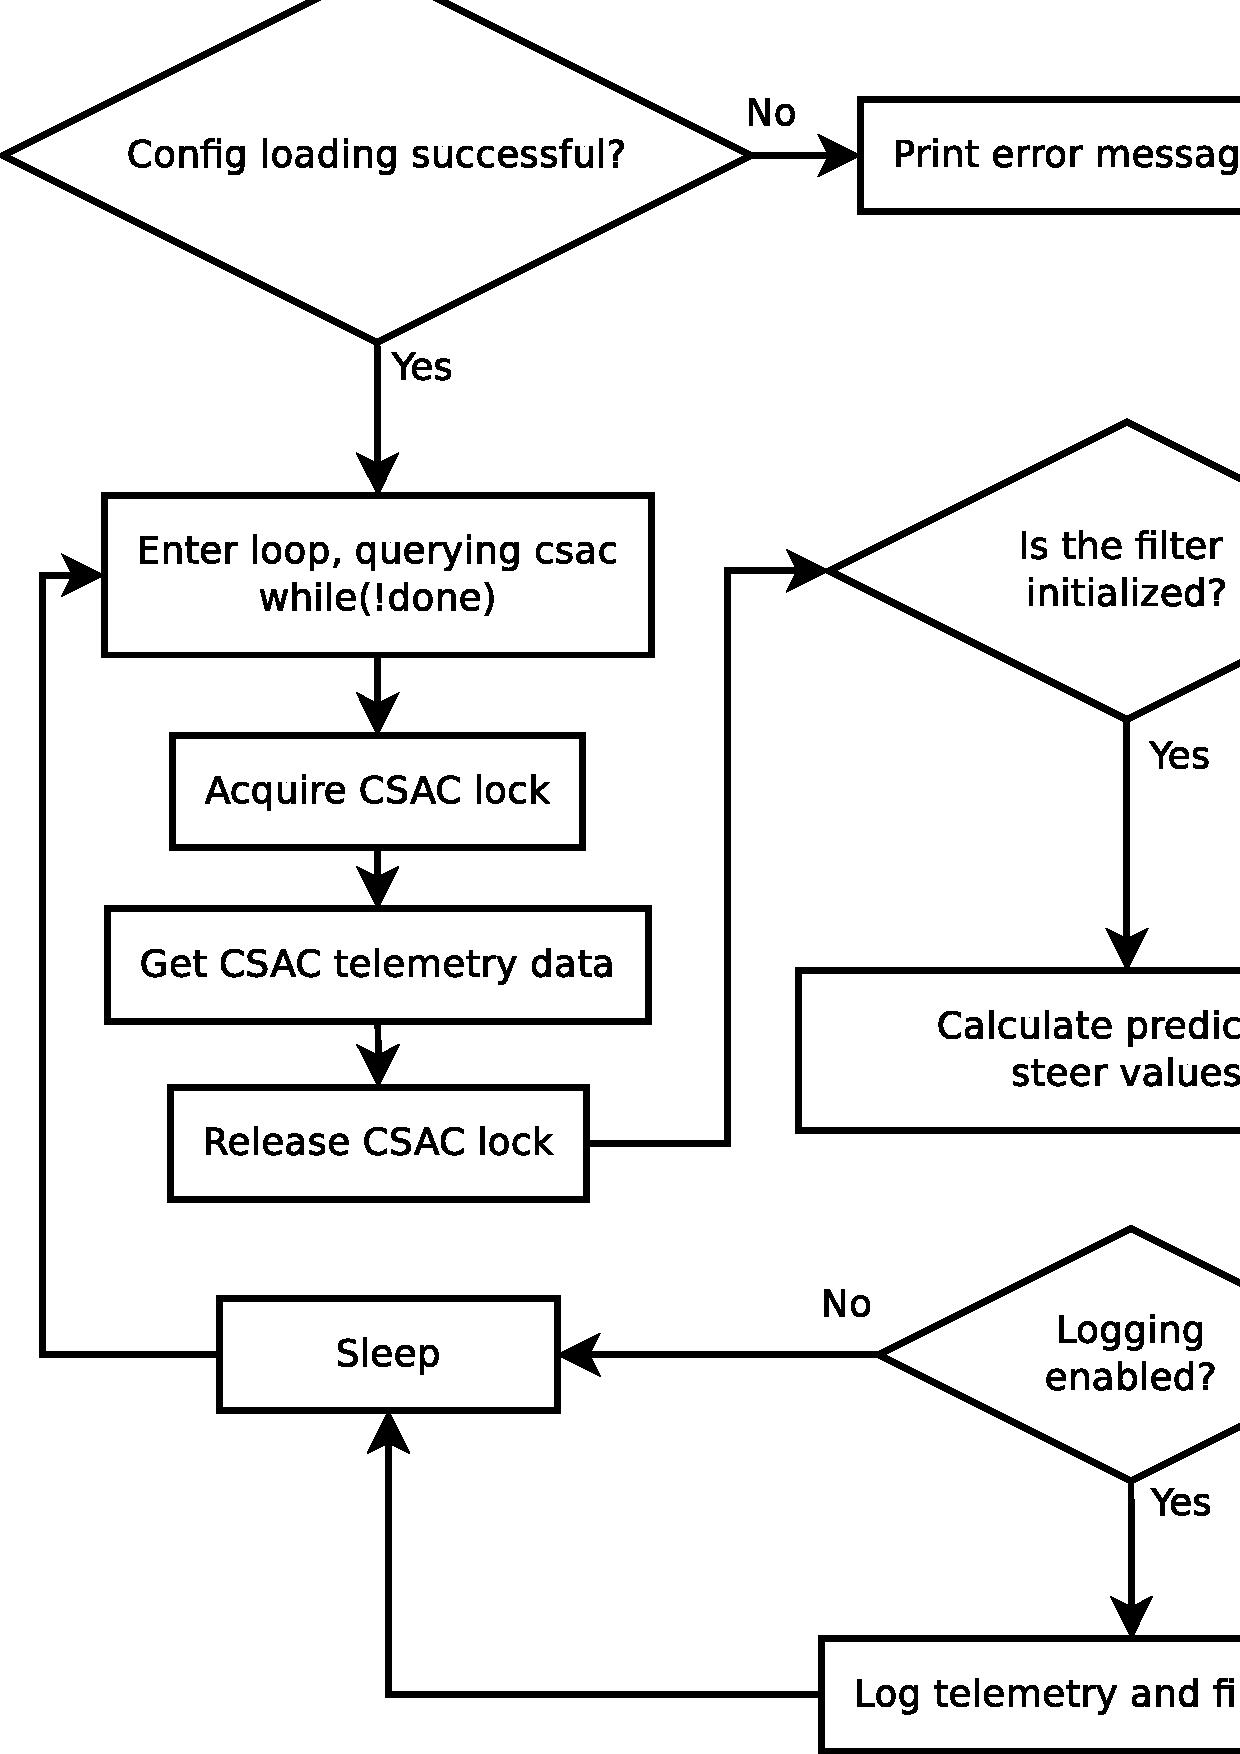
\includegraphics[angle=90, scale=0.40]{csac_filter.pdf}
   \caption[Socket Server execution flow block diagram]{The block diagram shows the execution flow of the CSAC filter.}
\end{figure}

\begin{figure}\label{actions_core}
\centering
  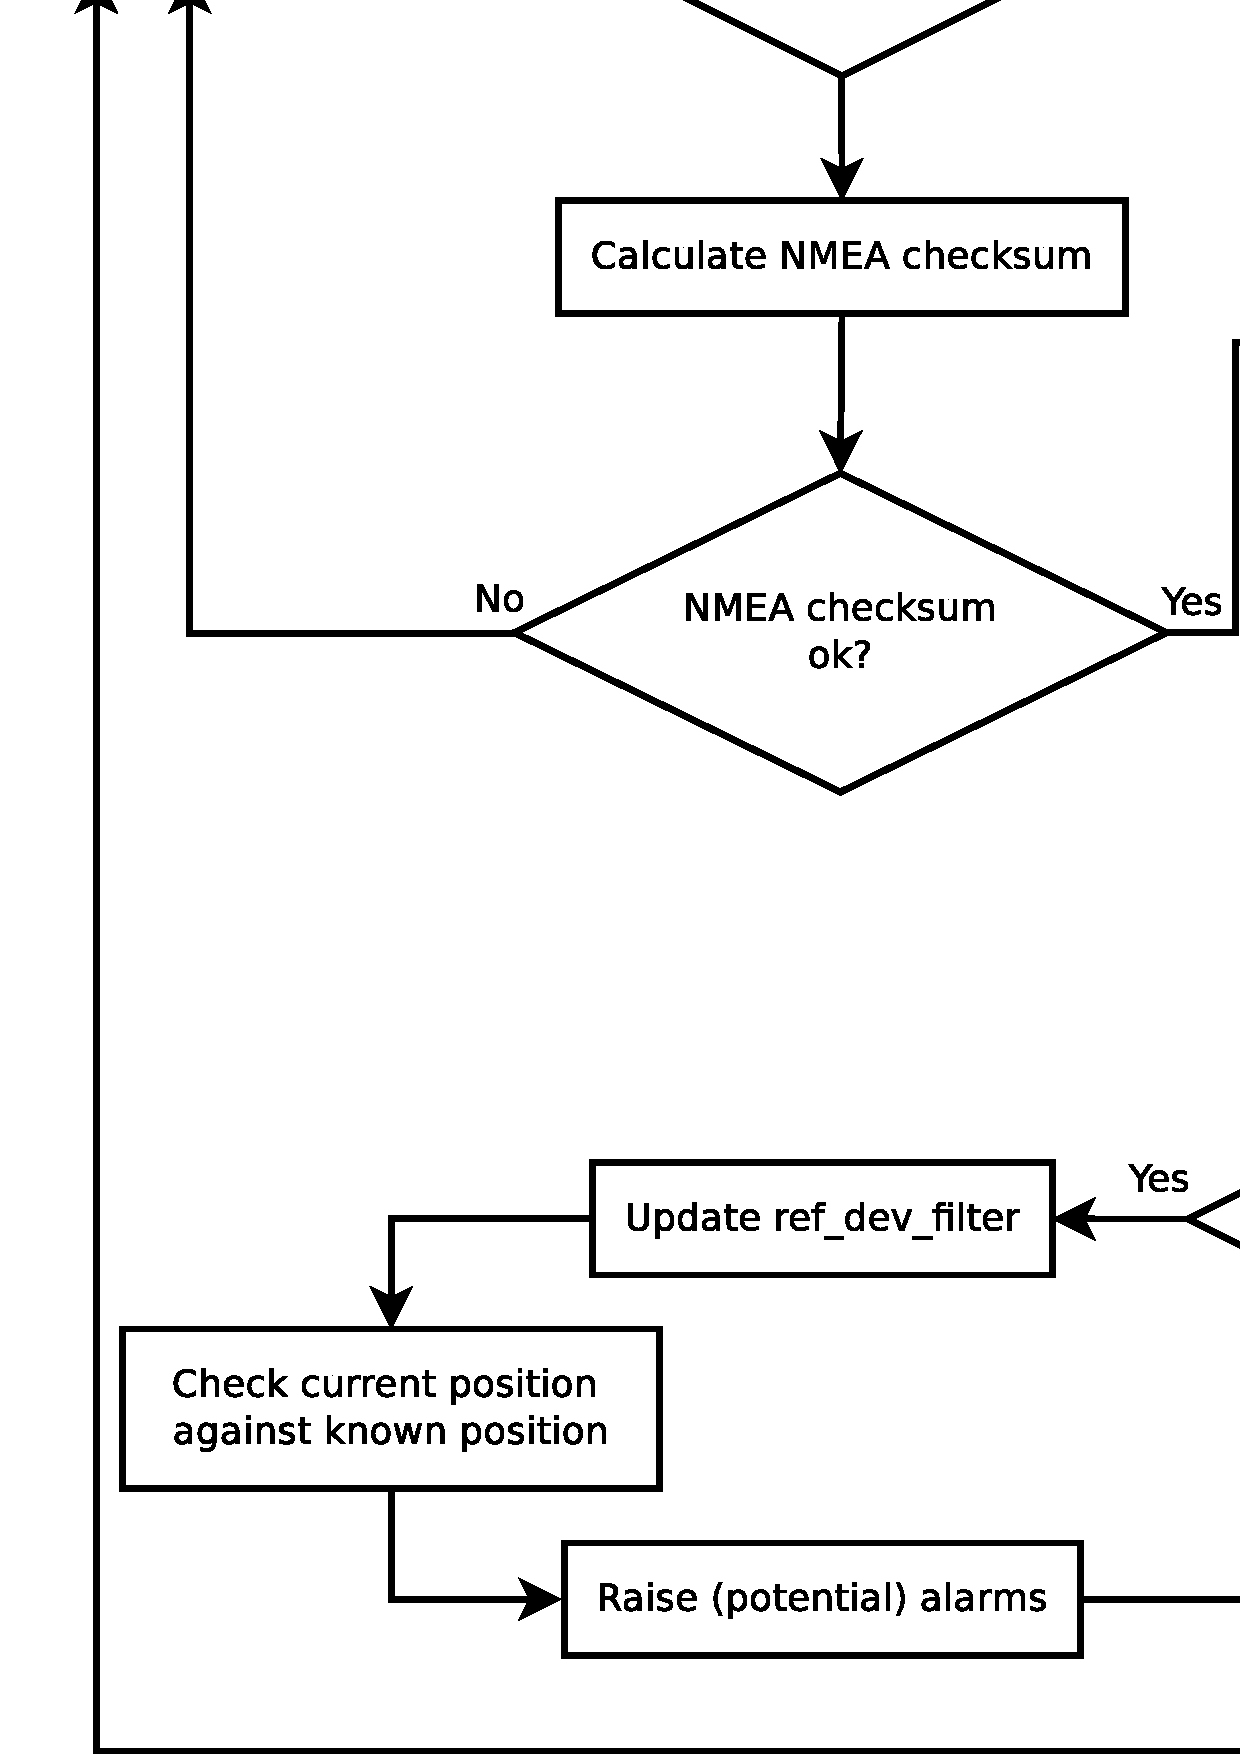
\includegraphics[scale=0.40]{actions_core.pdf}
   \caption[Socket Server execution flow block diagram]{The block diagrams shows and abstracted view of the execution after data has been received from a client.}
\end{figure}

\newpage
\subsection{Roles}
A client connected to the server can have two roles; It can either be a Sensor or a Monitor. The Sensor role is already explained, but the Monitor role was added in order for a user of the Sensor Server to connect to the server and check status or issue commands. For a client to assume the role of a Monitor, the client has to pick a negative integer as ID number. This way, the Server does not expect you as a client to report any NMEA data the way it would with a Sensor. As a Monitor, you can issue the following commands:

\begin{table}[!htb]
\centering
\caption{Sensor Server available commands}
\label{my-label}
\resizebox{1\textwidth}{!}{%
  \begin{tabular}{llll}
  \multicolumn{1}{l}{Command} & \multicolumn{1}{l}{Short} & \multicolumn{1}{l}{Parameter} & \multicolumn{1}{l}{Description}                                                                \\
  HELP                        & ?                         & NONE                          & Prints this table                                                                              \\
  IDENTIFY                    & ID                        & ID                            & Clients ID is set to PARAM                                                                     \\
  DISCONNECT                  & EXIT                      & NONE                          & Disconnect from the server                                                                     \\
  PRINTCLIENTS                & PC                        & NONE                          & Prints an overview of connected clients                                                        \\
  PRINTSERVER                 & PS                        & NONE                          & Prints server state and config                                                                 \\
  PRINTTIME                   &                           & ID                            & Prints time solved from GNSS data received from Sensor \textless ID\textgreater                 \\
  PRINTAVGDIFF                & PAD                       & NONE                          & Prints the difference between current solved position and the average reported for all Sensors \\
  PRINTLOC                    & PL                        & ID                            & Print solved position for Sensor \textless ID\textgreater                                       \\
  LISTDATA                    & LSD                       & NONE                          & List all dump files stored by the server                                                       \\
  DUMPDATA                    & DD                        & ID \& FILE                    & Dumps state of Sensor \textless ID\textgreater into a file named \textless FILE\textgreater      \\
  LOADDATA                    & LD                        & ID \& FILE                    & Load state stored in file called \textless FILE\textgreater into Sensor \textless ID\textgreater \\
  QUERYCSAC                   & QC                        & COMMAND                       & Queries the CSAC with COMMAND.                                                                 \\
  LOADRFDATA                  & LRFD                      & ID                            & Load reference location data into Sensor \textless ID\textgreater                               \\
  PRINTCFD                    & PFD                       & NONE                          & Prints CSAC filter data                                                                        
  \end{tabular}
}
\end{table}



\subsection{Sockets}
In order to implement the Server/Client model, the Sensor Server is implemented using the Linux Socket API. The API is based on BSD sockets and are available in in almost all Unix like operating system (\cite{LINUX_KERNEL}, p.610). Listing \ref{server_connect} shows a sample of code taken from one of the Sensor Server's source file. The sample shows the following:
\begin{itemize}
  \item Line 4: The server waits for a connection. \texttt{accept()} is a blocking function. The code does not continue past this point before a client has connected.  
  \item Line 12: The code has been executed way past the blocking \texttt{accept} function. Someone must have connected! The server forks out a new process from this point in the execution with the function \texttt{fork()}.
  \item Line 13: Upon entering the if statements regarding it's process identification (PID), the parent ends back at the top in the while loop. The child on the other hand, matches the criteria for the if sentence at line 15.
  \item Line 16: The child process closes it's parent's socket file descriptor and continues to setup the session at the next line.
\end{itemize}

\begin{code}
  \caption{Sample of code taken from \texttt{sensor\_server.c}(\ref{sensor_server.c}, line 356). The sample has been edited for clarity purposes.}
  \begin{minted}
  [
  fontsize=\footnotesize,
  fontfamily=tt,
  linenos=true
  ]
  {c}
    listen(server_sockfd,SOMAXCONN);
    int session_fd = 0;
    while (!done) {
        session_fd = accept(server_sockfd,0,0);
        if (session_fd==-1) {
            if (errno==EINTR) continue;
            t_print(ERROR_CONNECTION_ACCEPT,errno);
        }
        if(number_of_clients == max_clients) {
            close(session_fd);
        } else {
            pid_t pid=fork();
            if (pid==-1) {
                printf(ERROR_FAILED_FORK, errno);
            } else if (pid==0) {
                close(server_sockfd);
                setup_session(session_fd, new_client);
                close(session_fd);
                _exit(0);
            } else {
                close(session_fd);
            }
        }
    }
  \end{minted}
  \label{server_connect}
\end{code}
Even though the \texttt{accept()} function in the sockets API is blocking, CPU cycles are not wasted. If a socket call cannot be completed immediately, the process who issued the call will be put to sleep thus enabling the scheduler to schedule other processes for execution until conditions are right for the sleeping process. (\cite{UNIXN_WBA}, p.435). It is also possible to use non-blocking socket calls, and while this often increases performance, it also increases complexity, and was therefor not chosen for this approach. It's also worth mentioning that one could create \textit{threads} instead of forking out processes for new connections. The creation of threads are typically less expensive in terms of CPU cycles than the creation of processes. Processes on the other hand, always have their own virtual address space as opposed to threads who share their address space with the other threads withing the process. This makes programming with threads more complex and the result of a crash more severe as it affects the other threads as well. 

\subsection{Shared memory \& Semaphores}
The sensor server architecture uses several shared memory segments. This is necessary because as mentioned earlier(\ref{procvsthread}), each process has got it's own virtual address space. The pointers to the shared memory segments are declared as \textit{extern} in \texttt{sensor\_server.h}. The extern keyword means the the variable has an external linkage, making it visible from other files than the one in which it is defined. Listing \ref{extern_structs} shows a code sample taken from \texttt{sensor\_server.h} where the shared memory segments are declared.

\begin{code}
  \caption{Sample of code from \texttt{sensor\_server.h}(\ref{sensor_server.h}, line 356) where shared memory segments are declared.}
  \begin{minted}
  [
  fontsize=\footnotesize,
  fontfamily=tt,
  linenos=true
  ]
  {c}
    extern volatile sig_atomic_t done;
    extern struct client_table_entry *client_list;
    extern struct server_data *s_data;
    extern struct server_synchro *s_synch;
    extern struct server_config *s_conf;
    extern struct csac_filter_data *cfd;
  \end{minted}
  \label{extern_structs}
\end{code}

Every process that forks out from the server is given access to these memory segment. One might make the point that this voids the idea of processes, and one might be correct (see \ref{discussion}). The shared memory is created using the GNU library's Memory Mapped I/O (MMAP). Although typically used to map files to a region of memory, MMAP can also be used to create an anonymous map which is not connected to file but rather for sharing data between tasks without using files.

\begin{code}
  \caption{Listing shows the use of MMAP to create an anonymous map of memory to be used as a shared memory segment}
  \begin{minted}
  [
  fontsize=\footnotesize,
  fontfamily=tt,
  linenos=true
  ]
  {c}
  client_list = mmap(NULL, 
                    (s_conf->max_clients * sizeof(struct client_table_entry)), 
                    PROT_READ | PROT_WRITE,
                    MAP_SHARED | MAP_ANONYMOUS,
                    -1, 0);
  \end{minted}
\end{code}

Having shared memory segments comes with a price. Whenever two or more processes are working on the same data set, they are prone to create race conditions, deadlocks and data corruption. Therefore, semaphores where used to lock the segments during read and write operations at the shared memory segments.

\begin{code}
  \caption{Function for removing disconnected clients from list of clients}
  \begin{minted}
  [
  fontsize=\footnotesize,
  fontfamily=tt,
  linenos=true
  ]
  {c}
    void remove_client_by_id(int id)
    {
        struct client_table_entry* client_list_iterate;
        struct client_table_entry* temp_remove;

        sem_wait(&(s_synch->client_list_mutex));
        list_for_each_entry_safe(client_list_iterate, 
                                 temp_remove,&client_list->list,
                                 list) {
            if(client_list_iterate->client_id == id) {
                list_del(&client_list_iterate->list);
            }
        }
        s_data->number_of_clients--;
        sem_post(&(s_synch->client_list_mutex));
    }
  \end{minted}
  \label{removeclient}
\end{code}

Figure \ref{removeclient} shows a typical example of a function locking down access to the shared memory segment containing the list of connected clients, by using a semaphore. In the example (\ref{removeclient}) a client has been disconnected from the server and the the list of connected clients are being updated. The semaphore is necessary to make sure that another process is not attempting to read or write to the segment while the data is deleted. If another process had attempted to execute the \texttt{sem\_wait()} on the semaphore, it would have been put in a queue. Depending on the operating system, it would most likely signal the scheduler to do a context switch since the resource was busy anyway and it therefor should relinquish control of the CPU. Once the semaphores is raised, it can be lowered again by another process. It is important to note that the semaphores are not a function of or related to the memory segments by anything other the name. The semaphores are just "flags" used to control access to a resource. There is no automatic raising or lowering of the associated semaphores by reading or writing the shared memory segments. All functions in the sensor server does however use semaphores when dealing with shared memory segments in order to avoid deadlock and race conditions.

\subsection{Data structures}
In the C programming language, a "struct" is a complex data type that defines a list of variables to be placed under the structs given name in a block of memory. This makes it possible for multiple variables to be accessed via a single pointer. Before delving deeper into the code base of the sensor server, some crucial and often used structs will be explained in this section.

\subsubsection{Linked list}
Since the C standard does not provide data structures like linked lists, I had to choose between reinventing the wheel or finding some implementation to drop into the project. While studying another subject, I found a guide on how to use the linked list implementation from the linux kernel source code (\cite{KAZU_LIST}) in a user space program. Since the implementation was extremely solid, well tested and had many useful functions, i decided to use it. The modified header file containing all the code, is GPL licensed.  

\begin{code}
  \caption{Sample of code taken from \texttt{list.h} line 70}
    \begin{minted}
    [
    fontsize=\footnotesize,
    fontfamily=tt,
    linenos=true
    ]
    {c}
    struct list_head {
      struct list_head *next, *prev;
    };
    \end{minted}
    \label{struct_client_table}
\end{code}
The fields of the struct is pretty self explanatory. There is a pointer to previous node and one the next. By using these, the list can traversed. 

\subsubsection{client\_table\_entry}
The client\_table\_entry struct is what the name suggests, it's an entry in a list of clients. Every client connected to the server, no matter the purpose, has an entry in the client list. Listing \ref{struct_client_table} shows the complete struct. 

\begin{code}
  \caption{Sample of code taken from \texttt{sensor\_server\_common.h} line 99}
    \begin{minted}
    [
    fontsize=\footnotesize,
    fontfamily=tt,
    linenos=true
    ]
    {c}
    struct client_table_entry {
        struct list_head list; 
        struct transmission_s transmission; 
        struct timeval heartbeat_timeout; 
        struct command_code cm;   
        struct nmea_container nmea;    
        pid_t pid;  
        time_t timestamp;  
        int client_id; 
        int client_type;    
        int ready;  
        int marked_for_kick; 
        char ip[INET_ADDRSTRLEN];
        struct filters fs;
    };
    \end{minted}
    \label{struct_client_table}
\end{code}
The lient\_table\_entry struct is probably the type of the most commonly passed pointers in the program. 

\subsubsection{server\_config}
\begin{code}
  \caption{Sample of code taken from \texttt{sensor\_server.h} line 23}
    \begin{minted}
    [
    fontsize=\footnotesize,
    fontfamily=tt,
    linenos=true
    ]
    {c}
    struct server_config {
        int max_clients;
        int warm_up_seconds;
        int human_readable_dumpdata;
        char csac_path[PATH_LENGTH_MAX];
        int logging;
        char log_path[PATH_LENGTH_MAX];
        int csac_logging;
        char csac_log_path[PATH_LENGTH_MAX];
    };
    \end{minted}
    \label{struct_server_config} 
\end{code}

\subsubsection{server\_data}
\begin{code}
  \caption{Sample of code taken from \texttt{sensor\_server\_common.h} line 116}
    \begin{minted}
    [
    fontsize=\footnotesize,
    fontfamily=tt,
    linenos=true
    ]
    {c}
    struct server_synchro {
        sem_t ready_mutex;
        sem_t csac_mutex;
        sem_t client_list_mutex;
        volatile int ready_counter;
    };
    \end{minted}
  \label{server_data}
\end{code}

\subsubsection{server\_synchro}
\begin{code}
  \caption{Sample of code taken from \texttt{sensor\_server\_common.h} line 125}
    \begin{minted}
    [
    fontsize=\footnotesize,
    fontfamily=tt,
    linenos=true
    ]
    {c}
    struct server_synchro {
        sem_t ready_mutex;
        sem_t csac_mutex;
        sem_t client_list_mutex;
        volatile int ready_counter;
    };
    \end{minted}
  \label{server_synchro}
\end{code}

\subsubsection{command\_code}
\begin{code}
  \caption{Sample of code taken from \texttt{sensor\_server\_common.h} line 34}
    \begin{minted}
    [
    fontsize=\footnotesize,
    fontfamily=tt,
    linenos=true
    ]
    {c}
    struct command_code {
        int code;
        char parameter[MAX_PARAMETER_SIZE];
        int id_parameter;
    };
    \end{minted}
  \label{command_code}
\end{code}

\subsubsection{NMEA container}\label{nmea_cont}
\begin{code}
  \caption{Sample of code taken from \texttt{nmea.h} line 21}
    \begin{minted}
    [
    fontsize=\footnotesize,
    fontfamily=tt,
    linenos=true
    ]
    {c}
    struct nmea_container {
        /* Raw data */
        char raw_gga[SENTENCE_LENGTH];
        char raw_rmc[SENTENCE_LENGTH];

        /* Latitude */
        double lat_current;
        double lat_average;
        double lat_avg_diff;
        double lat_total;
        int lat_disturbed;

        /* Longitude */
        double lon_current;
        double lon_average;
        double lon_avg_diff;
        double lon_total;
        int lon_disturbed;

        /* Altitude */
        double alt_current;
        double alt_average;
        double alt_avg_diff;
        double alt_total;
        int alt_disturbed;

        /* Speed */
        double speed_current;
        double speed_average;
        double speed_avg_diff;
        double speed_total;
        int speed_disturbed;

        /* CHECKSUM */
        int checksum_passed;

        /* COUNTER FOR AVERAGE */
        int n_samples;
    };
    \end{minted}
    \label{nmea_container}
\end{code}

% Refer to protocol.h at the point when describing the ID process?
\section{The Sensor Client}\label{sensor_client}
The sensor client software is a simple program written in C99 whose only task is to relay information read from the GNSS receivers. Summed up shortly:
\begin{itemize}
  \item The client software takes two parameters to start, the servers IP and port. If parameters are missing, the program exits.
  \begin{itemize}
    \item Example: \texttt{./sensor\_client -p 10000 -i 192.168.1.5}
  \end{itemize}
  \item Initializes and loads configuration from configuration file. The configuration file includes path to the GNSS receiver, the sensors ID number and a binary value for whether or not logging of NMEA should be done as well as path to 
  the log file. If the loading of the configuration file fails, default values are used instead:
  \begin{itemize}
    \item The ID number is chosen at random but within legal limits.
    \item Logging is disabled.
    \item Maximum of server connection attempts are set to 10.
    \item Path to GNSS receiver is set to \texttt{/dev/ttyACM0}. This should be the path to the receiver unless another similar device is connected to the computer and given it is a Raspberry Pi running Raspbian.
  \end{itemize}
  \item Establishes communication with GNSS receiver, exits if it fails.
  \item Attempts to establish communication with the server, retries for a configurable amount of times at 1 second intervals.
  \item Identifies the client for the server according to protocol.
  \item Reads from the GNSS receiver, scans for lines starting with either \texttt{\$GNRMC} or \texttt{\$GNGGA}. When both lines are found, the data is stored in a buffer.
  \item Sends the GNSS data to the server according to protocol.
  \item Repeats.
\end{itemize}

\section{CSAC Communication}
  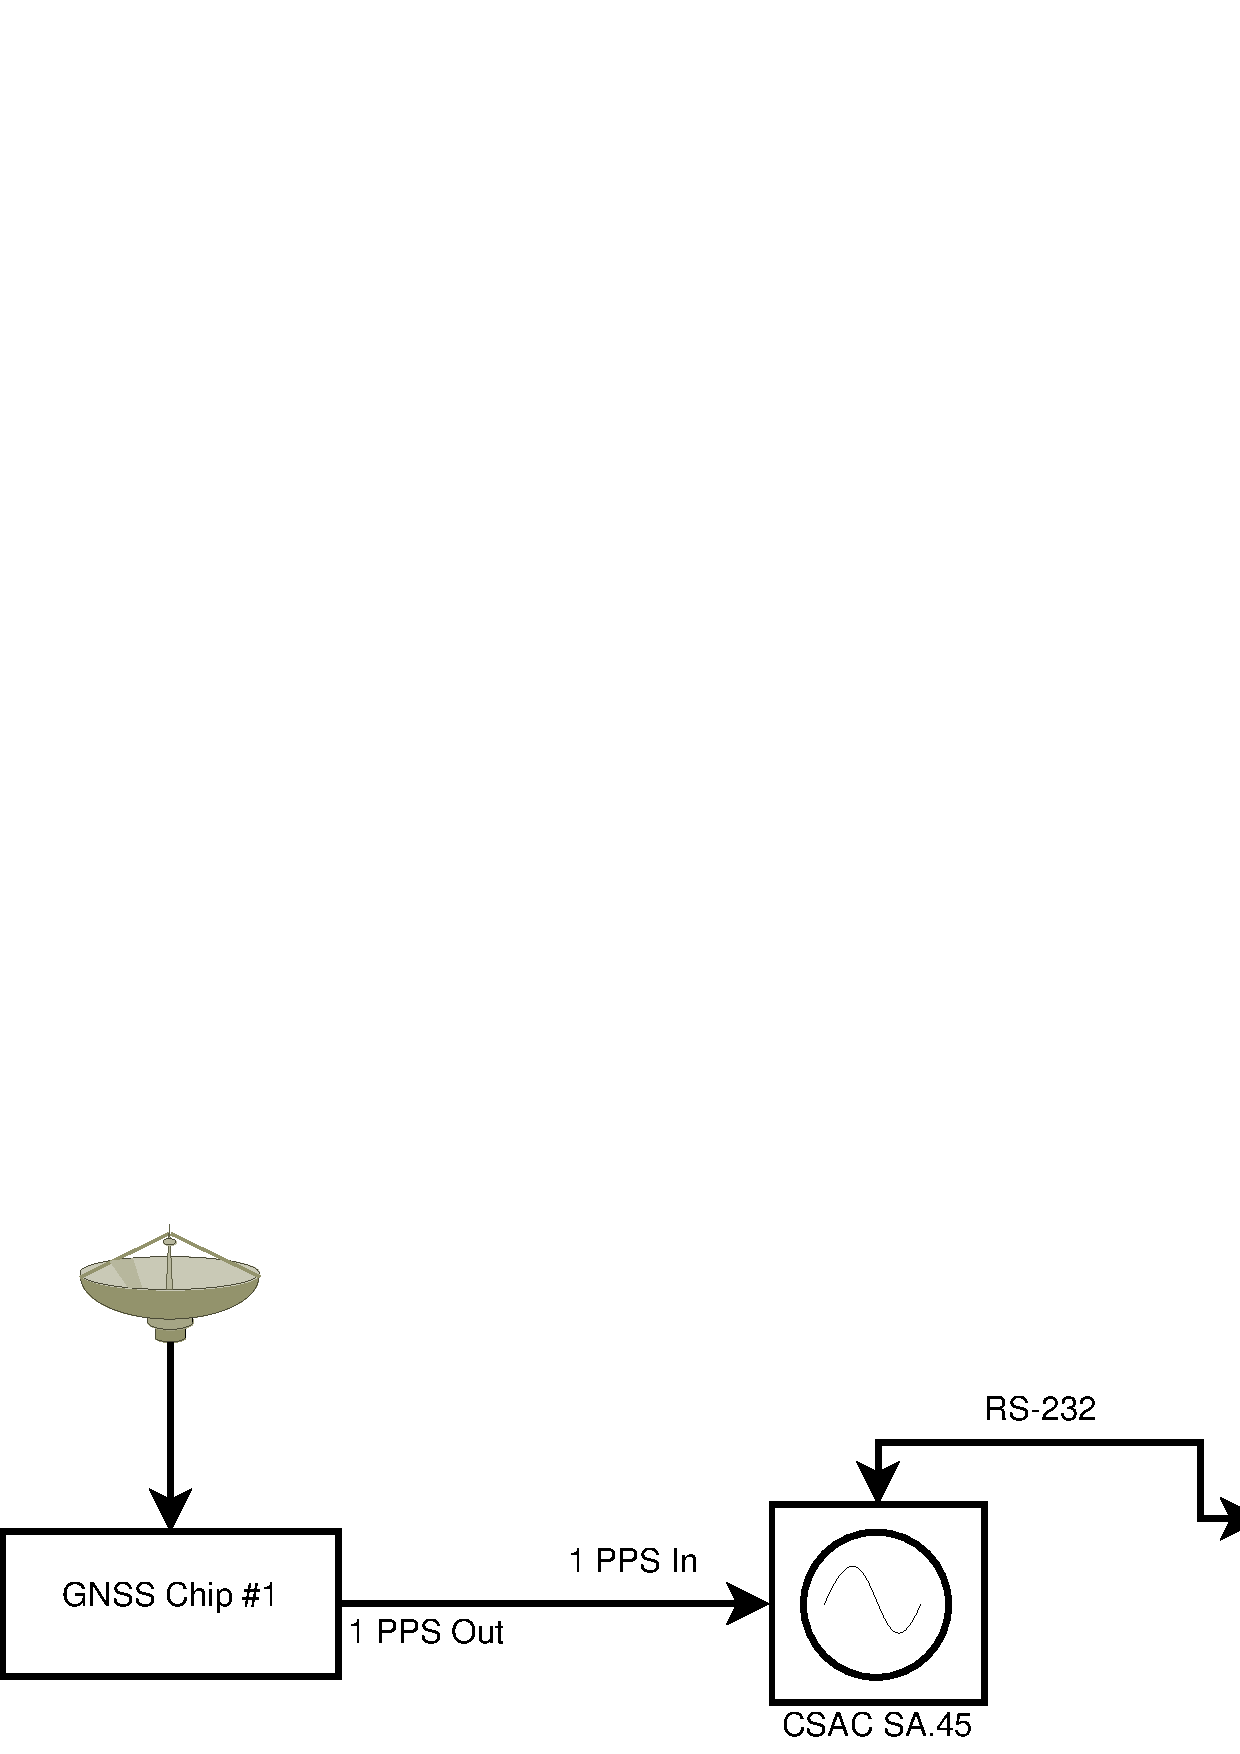
\includegraphics[width=1\textwidth]{csac_serial.pdf}
The SA.45 CSAC includes a serial interface that enables communication with a PC by using a COM port. As mentioned earlier, our approach relies heavily on the ability to communicate with the CSAC.
Information can be queried by sending commands to the CSAC. These commands are explained in table \ref{CSAC_COMMANDS}. 
\begin{table}[]
\centering
\caption{Commands for the SA.45 CSAC}
\label{CSAC_COMMANDS}
\begin{tabular}{|l|l|l|}
\hline
Shortcut          & Description                                        & Command                       \\ \hline
6                 & Return telemetry headers as comma-delimited string & !6{[}CRLF{]}                  \\ \hline
\textasciicircum  & Return telemetry as comma-delimited string         & !\textasciicircum  {[}CRLF{]} \\ \hline
F                 & Adjust frequency                                   & !F?{[}CRLF{]}                 \\ \hline
M                 & Set operating mode register bits                   & !M?{[}CRLF{]}                 \\ \hline
S                 & Sync CSAC 1 PPS to external 1 PPS                  & !S{[}CRLF{]}                  \\ \hline
D                 & Set 1 PPS disciplining time constant               & !D?{[}CRLF{]}                 \\ \hline
U                 & Set ultra-low power mode parameters                & !U?{[}CRLF{]}                 \\ \hline
T                 & Set/report time-of-day                             & !T?{[}CRLF{]}                 \\ \hline
\end{tabular}
\caption*{Source: \cite{CSAC_USERGUIDE}}
\end{table}

\section{Detection algorithms: Filters}
\subsection{Data acquisition}\label{data_aquisition}
In order to create an accurate clock-model of the CSAC, it was necessary to log data from it while it was running in a disciplined mode. In the disciplined mode, the CSAC will correct it's frequency based on either a 1 PPS (Pulse per second) signal or a 10 MHz signal. A similar approach was used in order to collect GPS data. Data from two u-blox NEO-M8T was gathered over the same time period as the data gathered from the CSAC. By gathering the data over the same period, it was possible to detect any correlation between the time solved by the GPS receivers and any frequency adjustments done by the CSAC. It also provided valuable data that could be used to tune the spoofing detection algorithms in the CSAC SMACC. The data gathering was done by simple Python scripts (\ref{CL} and \ref{GL}) running on a computer connected to the receivers and the CSAC (\ref{CLS})

\subsubsection{Clock Model (CM) based filter}\label{cmbf}
Write about clock model and the filters

\subsubsection{Known vs Reported location (KRL) filter}\label{kvsrlf}
As discussed during the introduction (\ref{cspakp}), an easy way to detect spoofing, is to check the GNSS receivers solved position against the known position of the receiver. The detection techniques efficiency also increases as more receivers are added to the detection setup. This is because it is hard to spoof a GNSS receiver without also spoofing it's neighbor. By accidentally spoofing the neighbor, the two GNSS receivers would solved the same position and position (depending on the spoofing technique), thus giving away the attempt. By configuring the Sensor Server with the location of the different Sensors, the server can act if Sensor reports an abnormal solved position. The filter is triggered when either latitude, longitude, altitude or speed is bigger or lower than the reference value minus or plus a deviation. Listing (\ref{ref_dev_filter_latitude}) shows an edited sample of code taken from \texttt{filters.c}. The code in the sample is part of the algorithm used to check whether or not the latitude part of the GNSS receivers solved position is within "safe" (not spoofed) range.
\begin{code}
  \caption{Sample of code taken from \texttt{filters.c} line 66. The code has been edited for clarity.}
    \begin{minted}
    [
      fontsize=\footnotesize,
      fontfamily=tt,
      linenos=true
    ]
    {c}
        if(latitude_current > latitude_reference + latitude_deviation) {
            moved = 1;
            lat_disturbed = HIGH;
        } else if(latitude_current < latitude_ref - latitude_dev) {
            moved = 1;
            latitude_disturbed = LOW;
        } else {
            latitude_disturbed = SAFE;
        }
    \end{minted}
    \label{ref_dev_filter_latitude}
\end{code}

\chapter{Testing}

\section{Spoofing simulation test}
When a GNSS receiver is spoofed, its solved position or time (or both) might change. The result depends on the technique used to spoof. By moving a GNSS receiver, one can simulate a spoofing attack since the location most certainly will change. It might also affect the time solved. (prat med Harald, dette er en problematisk forklaring). We also covered the antennas with aluminium foil to simulate a loss of signal. 

\subsection{Setup}
\begin{figure}
\centering
  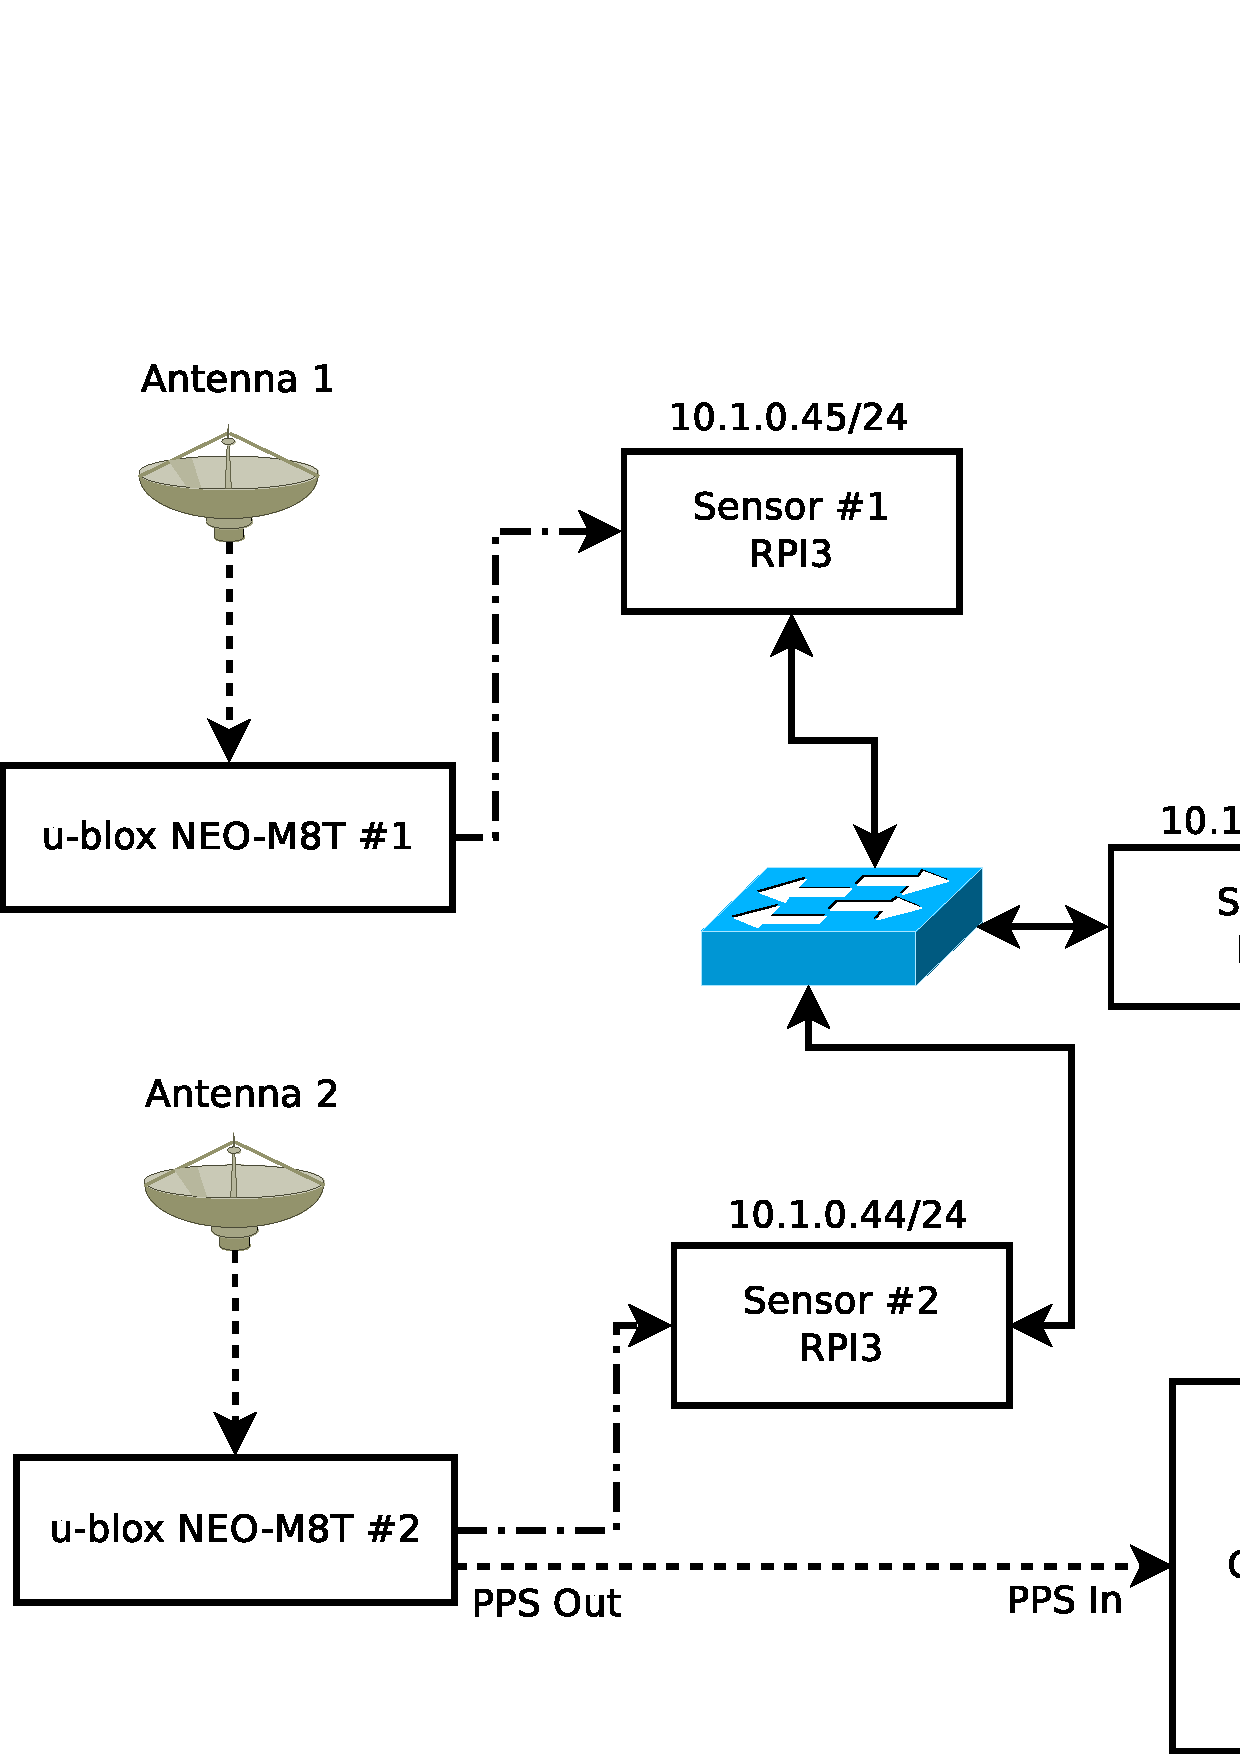
\includegraphics[scale=0.31]{server_layout.pdf}
   \caption[CSAC SMACC implementation block diagram]{A block diagram showing the tested implementation.}
   \label{ibd}
\end{figure}
Figure \ref{ibd} shows how the Server, Sensors and CSAC where physically set up. In order to assure good GNSS satellite geometry, the antennas where placed at a roof. Antenna 1 was placed at a railing about a 1 meter above the ground, antenna 2 was placed at ground level. Antenna 1 was connected to GNSS receiver 1 which in turn was connected to Sensor 1. It's the same setup with antenna 2 which was connected to GNSS receiver 2 which in turn was connected to Sensor 2. The distance between the two antennas was about 35 meters. The Sensors and the Server where connected to LAN through a Gigabit ethernet switch. The Server was configured to log telemetry received from the CSAC and the Clients where configured to log all NMEA data received from the GNSS receivers. The GNSS receiver connected to antenna South is used to supply the CSAC with a 1 PPS signal.

\begin{figure}
\centering
  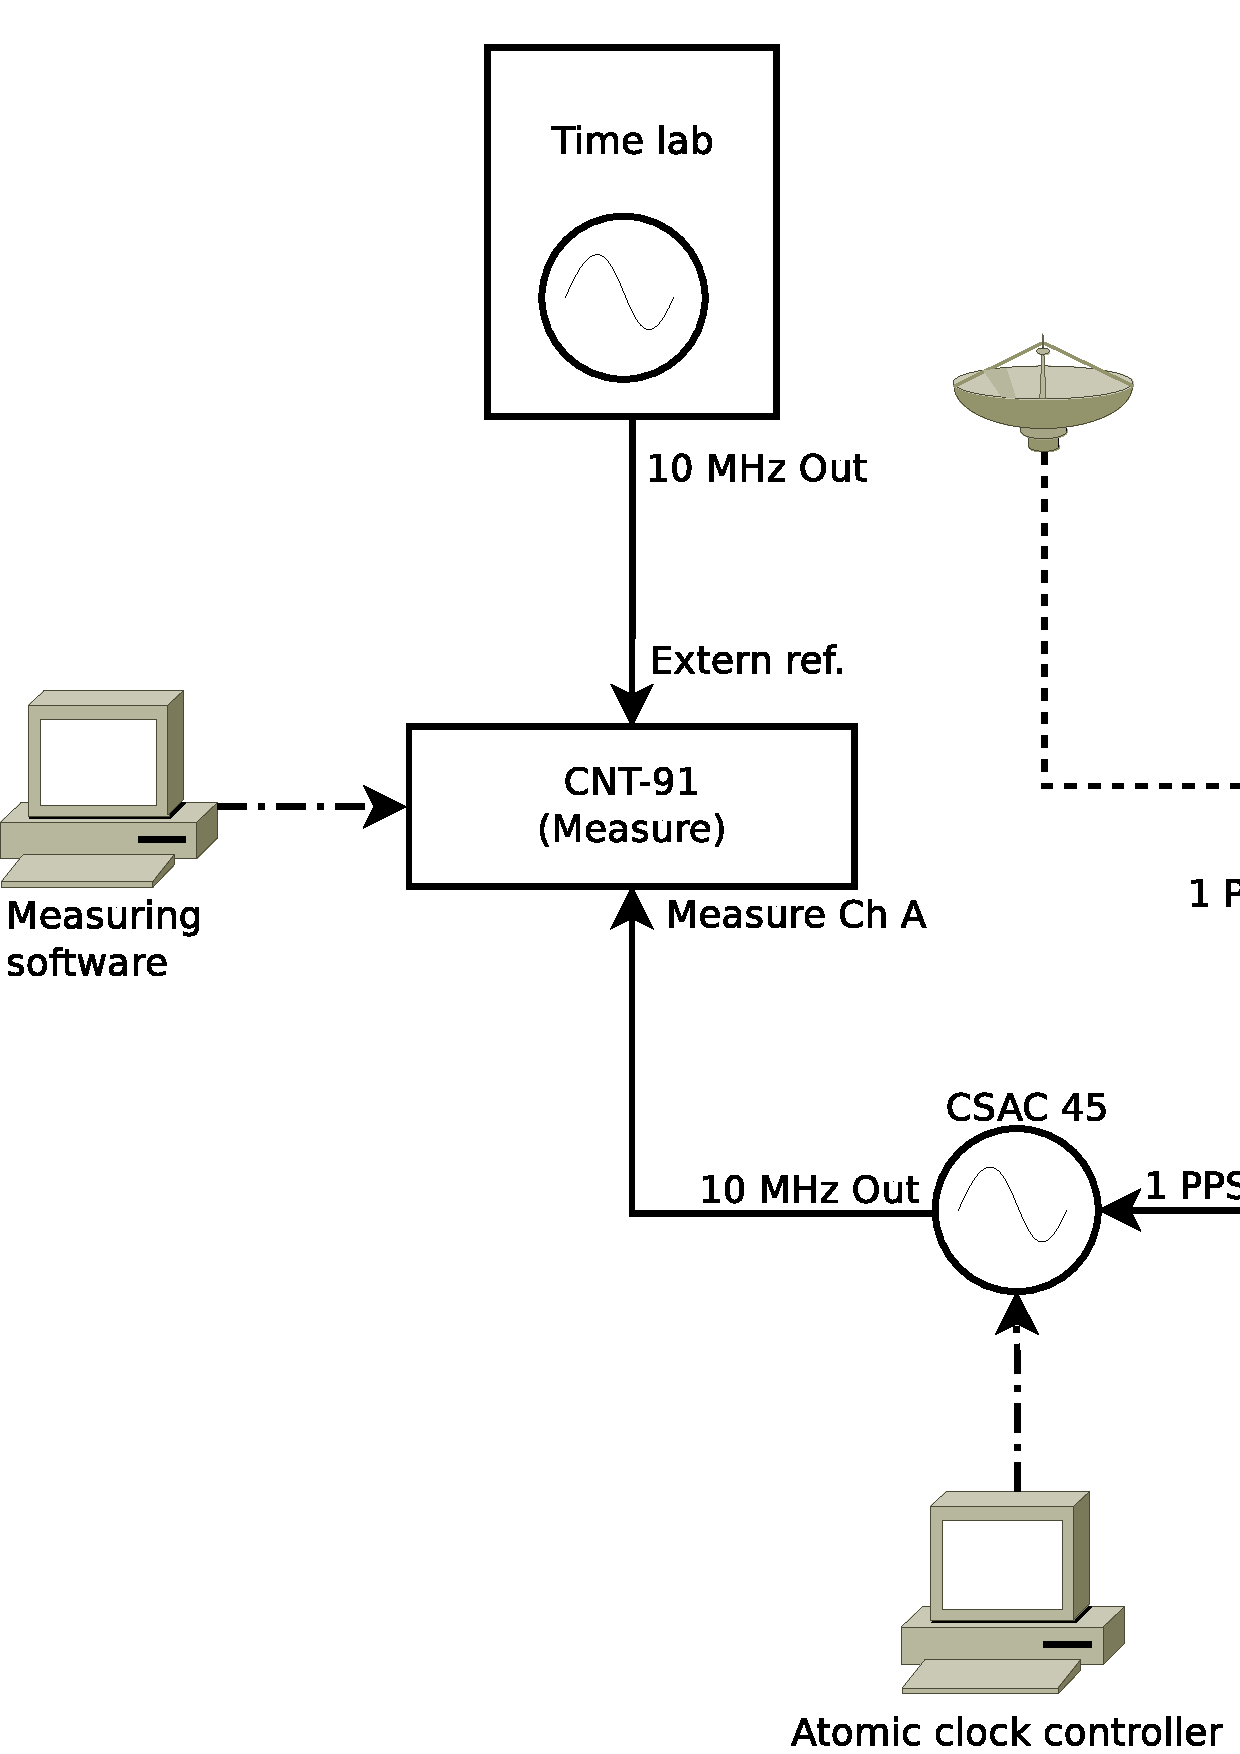
\includegraphics[scale=0.31]{measure_setup.pdf}
   \caption[Measurement setup]{Block diagram showing the setup of the measurement equipment}
   \label{msd}
\end{figure}
! DESCRIBE THE DETAILS OF THEM MEASUREMENT HERE !

\subsection{Goal}
The goal with this test was to use the CSAC SMACC to detect a simulated spoofing attack.

\subsection{Description}
The following is a step by step description of how the test was conducted.

\begin{itemize}
  \item 10:58, moved antenna 1 towards antenna 2.
  \item 11:03, moved antenna 1 back to original location.
  \item 11:07, moved antenna 2 towards antenna 1.
  \item 11:12, moved antenna 2 back to original location.
  \item 11:14, waved antenna 1 around at an increasing tempo.
  \item 11:18, waved antenna 1 around at an increasing tempo.
  \item 11:20, covered antenna 1 with aluminium foil. 
  \item 11:25, covered antenna 2 with aluminium foil. 
  \item 11:28, removed foil from antenna 1.
  \item 13:33, removed foil from antenna 2.
\end{itemize}

\subsection{Observations}
By reviewing the log produced by the Sensor Server, the following was observed:

\begin{itemize}
  \item The KRL (\ref{kvsrlf}) filter was triggered by Sensor 1 at 10:59:19 and cleared at 11:04:35.
  \begin{lstlisting}
    [10/10/16 - 10:59:17] [ ALARM ] Sensor 1 triggered KRL filter!
    ...
    [10/10/16 - 11:04:35] [ ALARM ] Sensor 1 cleared KRL filter!
  \end{lstlisting}
  \item The KRL (\ref{kvsrlf}) filter was triggered again at 11:08:27, but this time by Sensor 2. The alarm was cleared at 11:13:43.
    \begin{lstlisting}
    [10/10/16 - 11:08:27] [ ALARM ] Sensor 2 triggered KRL filter!
    ...
    [10/10/16 - 11:13:43] [ ALARM ] Sensor 2 cleared KRL filter!
  \end{lstlisting}
  \item Once again, 11:22:03 the KRL filter was triggered by Sensor 1 and was not cleared until 11:29:21
     \begin{lstlisting}
    [10/10/16 - 11:22:03] [ ALARM ] Sensor 1 triggered KRL filter!
    ...
    [10/10/16 - 11:29:21] [ ALARM ] Sensor 1 cleared KRL filter!
  \end{lstlisting} 
  \item At 11:27.05, it was the CM filter (\ref{cmbf}) using the clock model that triggered. It stopped triggering 11:27:33. Sensor 2 also triggered the KRL filter 11:27:31 and cleared at 11:34:16.
    \begin{lstlisting}
    [10/10/16 - 11:27:05] CSAC Steer current bigger than pred limit!
    ...
    [10/10/16 - 11:27:31] [ ALARM ] Sensor 2 triggered KRL filter!
    ...
    [10/10/16 - 11:27:33] [ ALARM ] CSAC Steer value greater than predicted!
  \end{lstlisting} 
  \item The last 6 seconds, Sensor 2 triggered KRL filter and the CM filter was triggered at multiple occasions.
  \begin{lstlisting}
    [10/10/16 - 11:34:15] , [ ALARM ] Sensor 2 triggered REF_DEV!
    [10/10/16 - 11:34:16] , [ ALARM ] Sensor 2 REF_DEV returned!
    [10/10/16 - 11:34:17] , [ ALARM ] Sensor 2 triggered REF_DEV!
    [10/10/16 - 11:34:18] , [ ALARM ] Sensor 2 triggered REF_DEV!
    [10/10/16 - 11:34:19] , [ ALARM ] Sensor 2 triggered REF_DEV!
    [10/10/16 - 11:34:19] ,Steer current bigger than pred limit!
    [10/10/16 - 11:34:20] ,Steer current bigger than pred limit!
    [10/10/16 - 11:34:20] , [ ALARM ] Sensor 2 REF_DEV returned!
    [10/10/16 - 11:34:21] ,Steer current bigger than pred limit!
  \end{lstlisting} 
\end{itemize}

\subsection{Conclusion}


\chapter{Results and discussion}\label{discussion}
\section{Choice of programming language}
The SMACC software was originally planned to be written in Java since this was my most fluent programming language. Java is great language, it's object oriented, it has a garbage collector and a lot of useful libraries. As development started, it quickly became apparent that some parts of the code would be performance critical and that portability really wasn't that important anyway. The platform was already decided and there was no reason to believe that it would change in the near future. As we all know, premature optimization is the root of all evil. Being reluctant to commit a deadly programming sin, i decided to look at other languages. Since performance was a concern, Python was also quickly dismissed as an option. C++ would probably have been the best choice, but having never written anything in C before made it sound more exciting and like a nice opportunity to learn something new. During the planning phase of SMACC development, raspbian-2015-05-07 was the latest build. It came with GCC 4.6.3 which only had experimental support for C11(\cite{GCC11}). With C11 no longer considered an option, C99 was the obvious choice given it's attractive features like:
\begin{itemize}
  \item Variable-length arrays.
  \item Single line comments.
  \item snprintf() as standard (\cite{C_RATIONAL}).
\end{itemize}


\section{Alternative approaches}\label{da}
When planning on how to execute our proposal, these where among the ideas that came up. 

\subsubsection{Single computer, many GNSS receivers}\label{scmgr}
A single computer is used to run the SMACC software. The SMACC does not include a Server/Cient model, but the receivers used to collect data are all connected to to the computer through whatever USB ports available or made available by the use of USB hubs. With this approach, you are not dependent on a network, but it limits the number of GNSS receivers you could connect as the USB specification limits the number possible endpoints to an absolute 127(\cite[pp. 3]{USBTC}) because of addressing. This does not mean that 127 devices can be connected, a single device might use more than one endpoint. It's also worth mentioning that a USB hub might "reserve" multiple endpoints. Depending on the GNSS receivers and how they are made, this number might be reduced even further by the power usage of the connected devices. Depending on how far each GNSS receiver is distanced from the SMACC, a signal amplifier might be necessary to compensate for the signal attenuation. In some cases where a network is absent, this might be only option.

\subsubsection{Store in database and analyze}
With this approach, the idea of a GNSS receiver and RASPI as a single "sensor" unit is the same as with Client-server approach. The difference is that it with this approach, each sensor stores the collected data in a database. The SMACC software monitors the clock directly as with the Client-server approach, but the data in the database is routinely queried and analyzed. The strength with this approach is that data is easily stored, shared and maintained by a single entity. The complexity of the client software would be the same as with Client-server approach, but the SMACC software could be implemented with less complexity as no Client-server architecture or shared memory schemes would be necessary. During planning, this approach seemed promising but was rejected because it was thought that it might not be time-sensitive enough. It was also some doubt concerning whether or not the ability to store data to a database actually was important. Once the different filters and algorithms was in place, it turned that the database functionality would have been nice, but not of any real importance for the SMACC to perform it's tasks, and would have been overkill anyway.

\chapter{Conclusion}
You should have done things different.

\subfile{appendix}

%===================================================

\newpage
\printbibliography[title={Complete Bibliography},heading=bibintoc]

\end{document}                    